\documentclass[border=6pt]{standalone}
\usepackage{amsmath,amssymb}
\usepackage{tikz}
\usetikzlibrary{decorations.pathreplacing,calc,positioning}
% TikZ styles and helpers shared by figures/circuits.tex and figures/circuits_qsvt.tex
\tikzset{
  wire/.style={line width=0.55pt},
  gate/.style={draw,fill=white,minimum height=6.2mm,minimum width=7.5mm,inner sep=1.5pt,font=\small,line width=0.55pt},
  wgate/.style={gate,minimum width=13mm},
  ctrl/.style={circle,fill=black,inner sep=0pt,minimum size=1.9mm},
  octrl/.style={circle,draw,fill=white,inner sep=0pt,minimum size=1.9mm,line width=0.55pt},
  targ/.style={circle,draw,inner sep=0pt,minimum size=3.2mm,line width=0.55pt},
  meter/.style={draw,fill=white,minimum height=6.2mm,minimum width=7.5mm,line width=0.55pt},
  reg/.style={font=\small,anchor=east},
  blk/.style={font=\footnotesize,anchor=north,text=black!65},
  st/.style={font=\footnotesize,anchor=south,text=blue!45!black},
  brace/.style={decorate,decoration={brace,mirror,amplitude=2.2pt},line width=0.4pt,black!60},
  slash/.style={},
}
\newcommand{\slashwire}[3]{% x y label : the /n mark on a multi-qubit wire
  \draw[line width=0.7pt] (#1cm-1.3mm,#2cm-1.6mm) -- (#1cm+1.3mm,#2cm+1.6mm);
  \node[font=\scriptsize,anchor=south west,inner sep=0.4pt] at (#1cm+0.9mm,#2cm+0.9mm) {#3};}
\newcommand{\vsep}[3]{% x ybot ytop : a dashed block boundary
  \draw[dashed,black!45,line width=0.4pt] (#1cm,#2cm) -- (#1cm,#3cm);}


% box spanning wires: x, ytop, ybot, width(cm), label
\newcommand{\mb}[5]{\draw[fill=white,line width=0.55pt] (#1-#4/2,#2+0.31) rectangle (#1+#4/2,#3-0.31); \node[font=\small] at (#1,{(#2+#3)/2}) {#5};}
\newcommand{\gt}[3]{\node[gate] at (#1,#2) {#3};}
\newcommand{\wg}[4]{\node[gate,minimum width=#3] at (#1,#2) {#4};}
\newcommand{\ct}[2]{\node[ctrl] at (#1,#2) {};}
\newcommand{\oc}[2]{\node[octrl] at (#1,#2) {};}
\newcommand{\vl}[3]{\draw[wire] (#1,#2) -- (#1,#3);}
\newcommand{\tg}[2]{\node[targ] at (#1,#2) {}; \draw[wire] (#1,#2-0.16) -- (#1,#2+0.16);}
\newcommand{\meas}[2]{\node[meter] at (#1,#2) {}; \draw[wire] (#1-0.25,#2-0.12) arc (160:20:0.27); \draw[wire,-latex] (#1,#2-0.12) -- (#1+0.2,#2+0.12);}
\newcommand{\wires}[3]{\foreach \y in {#3} {\draw[wire] (#1,\y) -- (#2,\y);}}
\newcommand{\lab}[3]{\node[reg] at (#1,#2) {#3};}
\definecolor{hitp}{RGB}{118,68,160}
\definecolor{classic}{RGB}{90,90,90}
\newcommand{\cbox}[6]{\draw[rounded corners=3pt,fill=black!4,draw=black!45,line width=0.5pt] (#1,#2) rectangle (#3,#4); \node[font=\footnotesize,align=center,text width=#6] at ({(#1+#3)/2},{(#2+#4)/2}) {#5};}
\begin{document}

\newcommand{\stg}[3]{\draw[densely dashed,black!35] (#1,#2) -- (#1,-2.05); \node[st] at (#1,#2) {#3};}
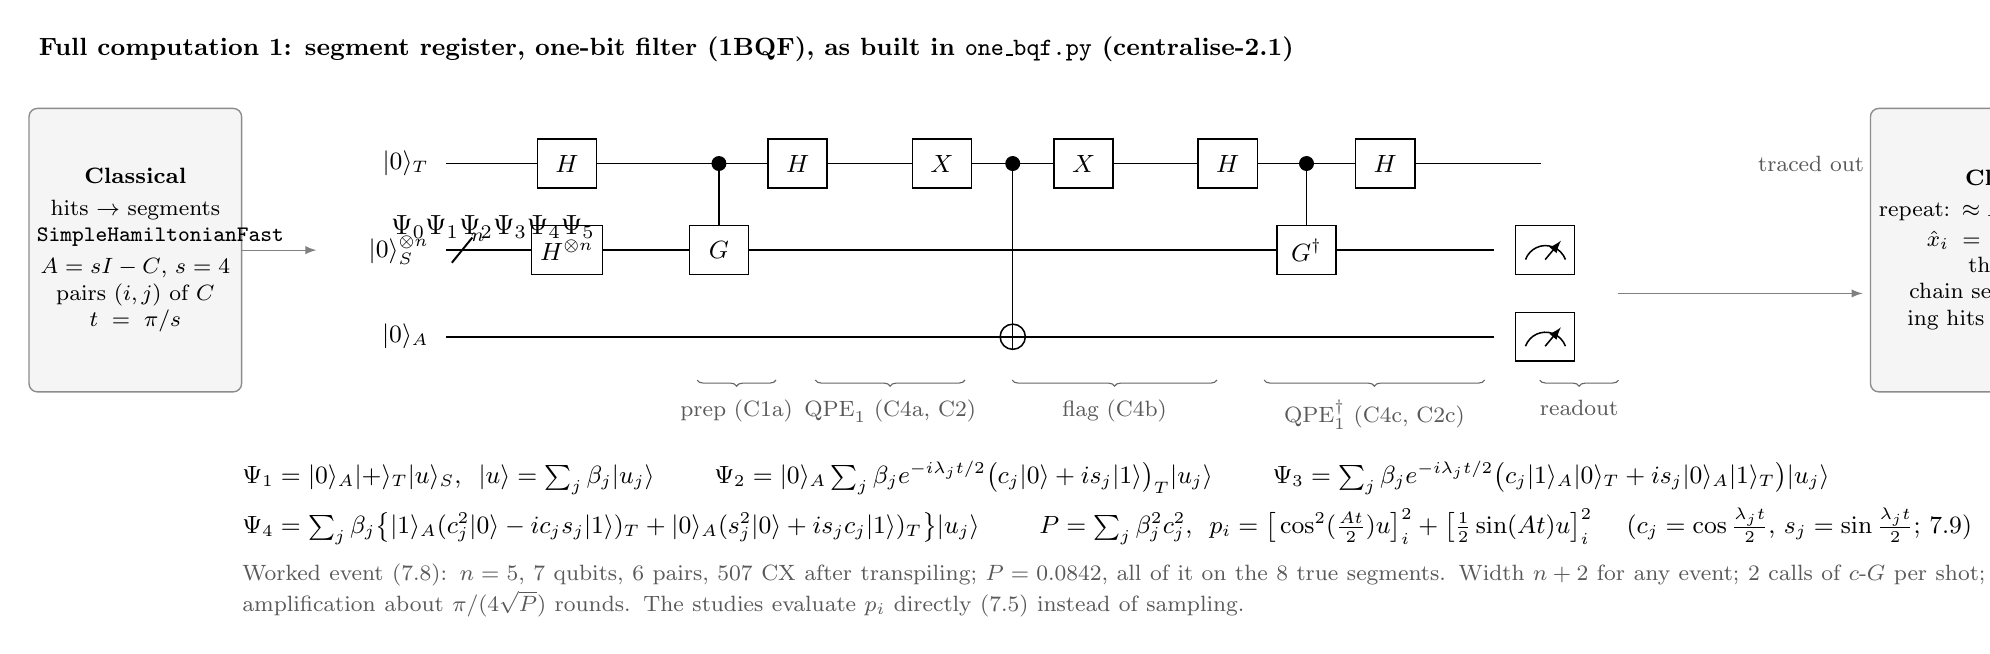
\begin{tikzpicture}[x=1cm,y=1cm]
\node[anchor=west,font=\small\bfseries] at (-4.6,2.35) {Full computation 1: segment register, one-bit filter (1BQF), as built in \texttt{one\_bqf.py} (centralise-2.1)};
% classical pre
\cbox{-4.6}{1.6}{-1.9}{-2.0}{\textbf{Classical}\\[2pt] hits $\to$ segments\\ \texttt{SimpleHamiltonianFast}\\[2pt] $A=sI-C$, $s=4$\\ pairs $(i,j)$ of $C$\\ $t=\pi/s$}{2.5cm}
\draw[-latex,black!50] (-1.9,-0.2) -- (-0.95,-0.2);
\lab{0.6}{0.9}{$|0\rangle_T$} \lab{0.6}{-0.2}{$|0\rangle^{\otimes n}_S$} \lab{0.6}{-1.3}{$|0\rangle_A$}
\wires{0.7}{14.6}{0.9} \wires{0.7}{14.0}{-0.2,-1.3} \slashwire{0.9}{-0.2}{$n$}
\stg{0.95}{1.35}{$\Psi_0$}
\gt{1.8}{0.9}{$H$} \wg{1.8}{-0.2}{9mm}{$H^{\otimes n}$}
\stg{2.55}{1.35}{$\Psi_1$}
\ct{3.3}{0.9} \vl{3.3}{0.9}{-0.2} \gt{3.3}{-0.2}{$G$} \gt{4.3}{0.9}{$H$}
\stg{5.0}{1.35}{$\Psi_2$}
\gt{5.7}{0.9}{$X$} \ct{6.6}{0.9} \vl{6.6}{0.9}{-1.3} \tg{6.6}{-1.3} \gt{7.5}{0.9}{$X$}
\stg{8.2}{1.35}{$\Psi_3$}
\gt{8.9}{0.9}{$H$} \ct{9.9}{0.9} \vl{9.9}{0.9}{-0.2} \gt{9.9}{-0.2}{$G^\dagger$} \gt{10.9}{0.9}{$H$}
\stg{11.6}{1.35}{$\Psi_4$}
\meas{12.5}{-0.2} \meas{12.5}{-1.3}
\stg{13.3}{1.35}{$\Psi_5$}
\node[font=\footnotesize,anchor=west,text=black!65] at (14.65,0.9) {traced out};
\draw[brace] (1.3,-1.85) -- (2.3,-1.85); \node[blk] at (1.8,-1.98) {prep (C1a)};
\draw[brace] (2.8,-1.85) -- (4.7,-1.85); \node[blk] at (3.75,-1.98) {$\mathrm{QPE}_1$ (C4a, C2)};
\draw[brace] (5.3,-1.85) -- (7.9,-1.85); \node[blk] at (6.6,-1.98) {flag (C4b)};
\draw[brace] (8.5,-1.85) -- (11.3,-1.85); \node[blk] at (9.9,-1.98) {$\mathrm{QPE}_1^\dagger$ (C4c, C2c)};
\draw[brace] (12.0,-1.85) -- (13.0,-1.85); \node[blk] at (12.5,-1.98) {readout};
\draw[-latex,black!50] (13.0,-0.75) -- (16.1,-0.75);
\cbox{16.2}{1.6}{19.9}{-2.0}{\textbf{Classical}\\[2pt] repeat: $\approx M\ln M/P$ shots\\ $\hat x_i=\sqrt{n_i/n_{\rm succ}}$\\ threshold\\ chain segments sharing hits (\texttt{get\_tracks})}{3.5cm}
% stage formulas
\node[font=\small,anchor=north west,text width=24.3cm,align=left] at (-4.6,-2.75) {\raggedright 
$\Psi_1=|0\rangle_A|{+}\rangle_T|u\rangle_S$, \ $|u\rangle=\sum_j\beta_j|u_j\rangle$ \qquad
$\Psi_2=|0\rangle_A\sum_j\beta_je^{-i\lambda_jt/2}\big(c_j|0\rangle+is_j|1\rangle\big)_T|u_j\rangle$ \qquad
$\Psi_3=\sum_j\beta_je^{-i\lambda_jt/2}\big(c_j|1\rangle_A|0\rangle_T+is_j|0\rangle_A|1\rangle_T\big)|u_j\rangle$\\[4pt]
$\Psi_4=\sum_j\beta_j\big\{|1\rangle_A(c_j^2|0\rangle-ic_js_j|1\rangle)_T+|0\rangle_A(s_j^2|0\rangle+is_jc_j|1\rangle)_T\big\}|u_j\rangle$ \qquad
$P=\sum_j\beta_j^2c_j^2$, \ $p_i=\big[\cos^2(\tfrac{At}{2})u\big]_i^2+\big[\tfrac12\sin(At)u\big]_i^2$ \quad ($c_j=\cos\tfrac{\lambda_jt}{2}$, $s_j=\sin\tfrac{\lambda_jt}{2}$; 7.9)\\[6pt]
\footnotesize\color{black!65} Worked event (7.8): $n=5$, 7 qubits, 6 pairs, 507 CX after transpiling; $P=0.0842$, all of it on the 8 true segments. Width $n+2$ for any event; 2 calls of $c\text{-}G$ per shot; with amplitude amplification about $\pi/(4\sqrt P)$ rounds. The studies evaluate $p_i$ directly (7.5) instead of sampling.};
\end{tikzpicture}
\end{document}
